\documentclass[12pt,a4paper]{article}
\usepackage[utf8]{inputenc}
\usepackage{dsfont} 
\usepackage[polish]{babel}
\usepackage{amsmath}
\usepackage{graphicx}
\usepackage[top=1in, bottom=1.5in, left=1.25in, right=1.25in]{geometry}
\usepackage{pdfpages}
\usepackage{subfig}
\usepackage{multirow}
\usepackage{multicol}
\graphicspath{{Imagens/}}
\usepackage{xcolor,colortbl}
\usepackage{float}
\usepackage[T1]{fontenc}

\newcommand \comment[1]{\textbf{\textcolor{red}{#1}}}

\usepackage{fancyhdr} % Required for custom headers
\usepackage{lastpage} % Required to determine the last page for the footer
\usepackage{extramarks} % Required for headers and footers
\usepackage{indentfirst}
\usepackage{placeins}
\usepackage{scalefnt}
\usepackage{xcolor,listings}
\usepackage{textcomp}
\usepackage{color}
\usepackage{verbatim}
\usepackage{framed}

\definecolor{codegreen}{rgb}{0,0.6,0}
\definecolor{codegray}{rgb}{0.5,0.5,0.5}
\definecolor{codepurple}{HTML}{C42043}
\definecolor{backcolour}{HTML}{F2F2F2}
\definecolor{bookColor}{cmyk}{0,0,0,0.90}  
\color{bookColor}

\lstset{upquote=true}

\lstdefinestyle{mystyle}{
	backgroundcolor=\color{backcolour},   
	commentstyle=\color{codegreen},
	keywordstyle=\color{codepurple},
	numberstyle=\numberstyle,
	stringstyle=\color{codepurple},
	basicstyle=\footnotesize\ttfamily,
	breakatwhitespace=false,
	breaklines=true,
	captionpos=b,
	keepspaces=true,
	numbers=left,
	numbersep=10pt,
	showspaces=false,
	showstringspaces=false,
	showtabs=false,
}
\lstset{style=mystyle}

\newcommand\numberstyle[1]{%
	\footnotesize
	\color{codegray}%
	\ttfamily
	\ifnum#1<10 0\fi#1 |%
}

\definecolor{shadecolor}{HTML}{F2F2F2}

\newenvironment{sqltable}%
{\snugshade\verbatim}%
{\endverbatim\endsnugshade}

% Margins
\addtolength{\footskip}{0cm}
\addtolength{\textwidth}{1.4cm}
\addtolength{\oddsidemargin}{-.7cm}

\addtolength{\textheight}{1.6cm}
%\addtolength{\topmargin}{-2cm}

% paragrafo
\addtolength{\parskip}{.2cm}

% Set up the header and footer
\pagestyle{fancy}
\rhead{\hmwkAuthorName} % Top left header
\lhead{\hmwkClass: \hmwkTitle} % Top center header
\rhead{\firstxmark} % Top right header
\lfoot{Damian Pawłowski} % Bottom left footer
\cfoot{} % Bottom center footer
\rfoot{} % Bottom right footer
\renewcommand{\headrulewidth}{1pt}
\renewcommand{\footrulewidth}{1pt}

    
\newcommand{\hmwkTitle}{Schemat systemu informatycznego obsługującego system wirtualnej uczelni} % Tytuł projektu
\newcommand{\hmwkDueDate}{\today} % Data 
\newcommand{\hmwkClass}{Bazy danych} % Nazwa przedmiotu
\newcommand{\hmwkAuthorName}{Damian Pawłowski} % Imię i nazwisko

% trabalho 
\begin{document}
% capa
\begin{titlepage}
    \vfill
	\begin{center}
	\hspace*{-1cm}
	\vspace*{0.5cm}
    
\includegraphics[scale=0.55]{imagens/loga.png}\\
	\textbf{Uniwersytet Gdański \\ [0.05cm]Wydział Matematyki, Fizyki i Informatyki \\ [0.05cm] Instytut Informatyki}

	\vspace{0.6cm}
	\vspace{4cm}
	{\huge \textbf{\hmwkTitle}}\vspace{8mm}
	
	{\large \textbf{\hmwkAuthorName}}\\[3cm]
	
		\hspace{.45\textwidth} %posiciona a minipage
	   \begin{minipage}{.5\textwidth}
	   Projekt z przedmiotu bazy danych na kierunku informatyka profil ogólnoakademicki na Uniwersytecie Gdańskim.\\[0.1cm]
	  \end{minipage}
	  \vfill
	%\vspace{2cm}
	
	\textbf{Gdańsk}
	
	\textbf{\hmwkDueDate}
	\end{center}
	
\end{titlepage}

\newpage

\setcounter{secnumdepth}{5}
\tableofcontents

\newpage

\section{Wprowadzenie}
\label{sec:introduction}

Baza danych przeznaczona jest dla szkoły wyższej.

Ma ona na celu zmodernizowanie szkoły za pomocą elektronicznego sposobu przechowywania danych.

Ułatwi ona dokumentację najważniejszych informacji takich jak oceny czy wpłaty.

Umożliwi ona dostęp do internetowego planu lekcji dla studentów oraz nauczycieli.

Baza znajdować się będzie na zewnętrznym serwerze.

Baza jest znormalizowana do 3 Postaci Normalnej.

\section{Opis projektu}
\label{sec:Project}

Taka baza to idealne rozwiązanie dla nowo powstałej lub staroświeckiej uczelni.

Umożliwia ona zastąpienie tradycyjnego papierowego dziennika znacznie nowocześniejszym.

Pozwala ona na bezpieczne przechowywanie informacji o studentach , nauczycielach , ocenach , akademikach , wykładach oraz o pozostałych rzeczach związanych z funkcjonowaniem szkoły.

System umożliwia błyskawiczne liczenie średnich uczniów, porównywanie najlepszych ocen, szybkie sprawdzanie danych.

\subsection{Potencjalne grupy użytkowników}
\label{sec:Users}

\begin{itemize}
	\item Administrator – Główny zarządca bazy danych, posiada pełen dostęp do bazy danych.
	\item Pracownicy uczelni – Mają dostęp do informacji o uczniach,ocenach,salach,planach lekcji.
	\item Studenci – Mają dostęp do swoich ocen,wpłat,świadczeń oraz informacji ogólnodostępnych o uczelni.
	\item Goście – Mają dostęp do informacji ogólnodostępnych np o kierunkach uczelni czy akademikach.
\end{itemize}

\newpage
\subsection{Wymagania funkcjonalne}
\label{sec:FunctionalConditions}

Baza będzie przechowywać dane osobowe, adresy , oceny , cenniki , informacje o wydziałach, telefony , adresy email , pensje , daty.
Jej zadania:
\begin{itemize}
	\item tworzenie planow lekcji
	\item monitorowanie ocen
	\item wyswietlanie inf. o studentach i nauczycielach
	\item wyswietlanie inf. pracach dyplomowych
	\item wyswietlanie inf. akademikach
	\item dokumentowanie wplat oraz swiadczen
\end{itemize}

\subsection{Wymagania niefunkcjonalne}
\label{sec:NonFunctionalConditions}
Baza znajduje się na zewnętrznym serwerze freemysqlhosting.net.
Jego największą zaletą jest to, że jest za darmo.
Darmowa wersja posiada pewne ograniczenie pamięci.
Lecz zawsze można ulepszyć ją do wersji płatnej.
Jeśli jest to nowa szkoła to takie rozwiązanie będzie najlepsze na kilka pierwszych miesięcy.

Do danych serwera można dostać się za pomocą phpmyadmin.

System zarządzania bazą danych to MySql 5.0.

Do jego zalet należą: 
\begin{itemize}
	\item Solidność
	\item Innowacyjność
	\item Łatwość w obsłudze
	\item Szybkość
	\item Open-Source
\end{itemize}

Do wad można zaliczyć:

\begin{itemize}
	\item Mniejszy poziom zaawansowania niż inne systemy takie jak np. PostSQL
\end{itemize}

\subsection{Diagram związków encji}
\label{sec:ERD} 

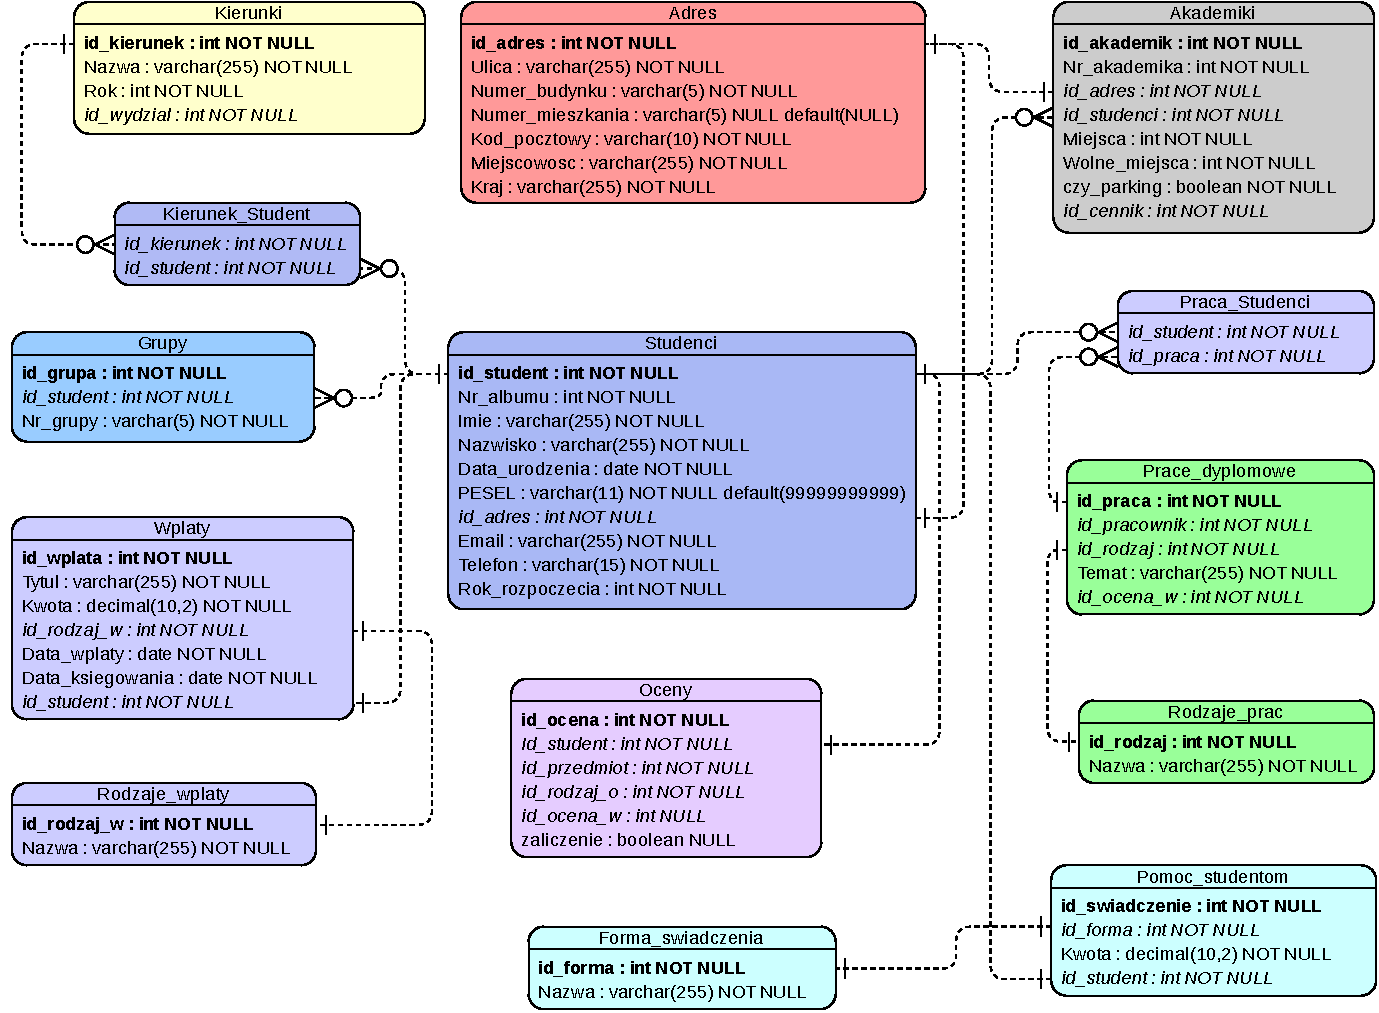
\includepdf[lastpage=1]{erd1.pdf}
\newpage
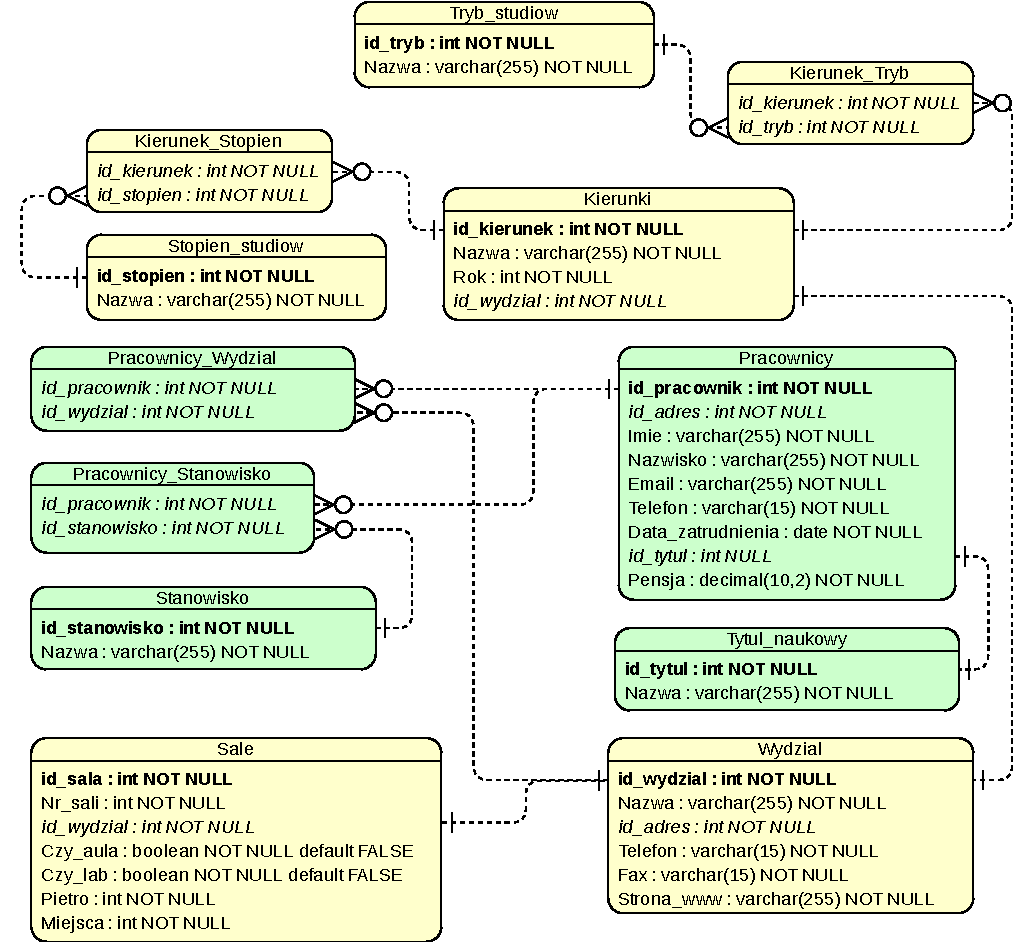
\includepdf[lastpage=1]{erd2.pdf}
\newpage
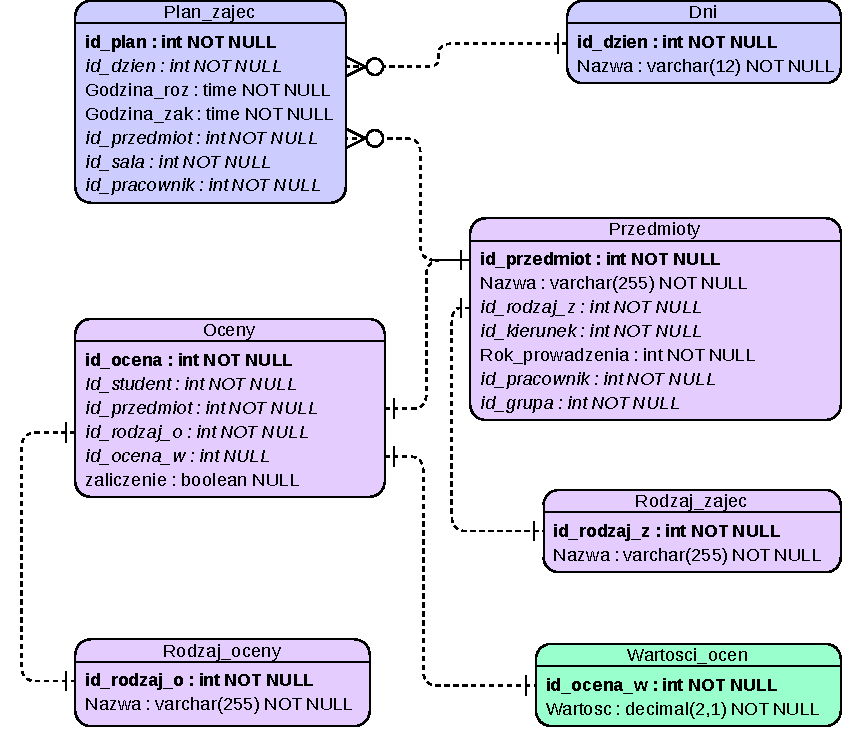
\includepdf[lastpage=1]{erd3.pdf}
\newpage
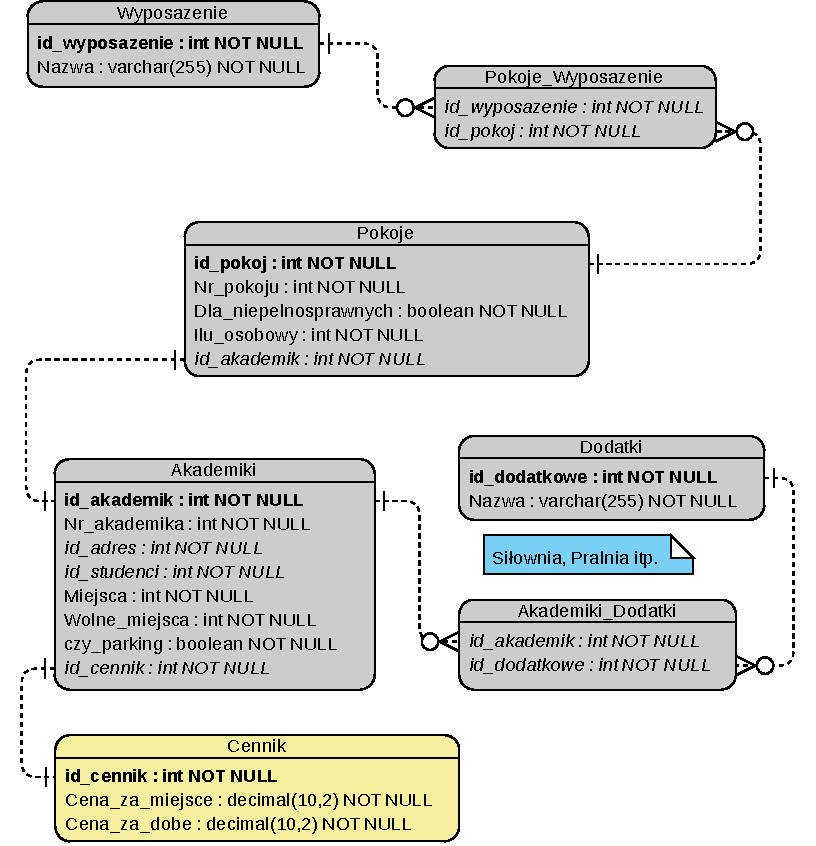
\includepdf[lastpage=1]{erd4.pdf}

\section{Przykłady realizacji bazy danych}
\label{sec:ExamplesSection}

Poniższe przykłady są w formie tabel SQL uzyskanych za pomocą polecenia DESCRIBE, oraz zapytań SQL i ich wyników.

\subsection{Przykłady zawartości najważniejszych tabel}
\label{sec:ExampleTables}

\textbf{Tabela STUDENCI:}

\begin{sqltable}
+-----------------+--------------+------+-----+-------------+-------+
| Field           | Type         | Null | Key | Default     | Extra |
+-----------------+--------------+------+-----+-------------+-------+
| id_student      | int(11)      | NO   | PRI | NULL        | A_I   |
| nr_albumu       | int(11)      | NO   |     | NULL        |       |
| imie            | varchar(255) | NO   |     | NULL        |       |
| nazwisko        | varchar(255) | NO   |     | NULL        |       |
| data_urodzenia  | date         | NO   |     | NULL        |       |
| pesel           | varchar(11)  | NO   | UNI | 99999999999 |       |
| id_adres        | int(11)      | NO   |     | NULL        |       |
| email           | varchar(255) | NO   |     | NULL        |       |
| telefon         | varchar(15)  | NO   |     | NULL        |       |
| rok_rozpoczecia | int(11)      | NO   |     | NULL        |       |
+-----------------+--------------+------+-----+-------------+-------+
\end{sqltable}

\textbf{Tabela ADRES:}

\begin{sqltable}
+------------------+--------------+------+-----+---------+-------+
| Field            | Type         | Null | Key | Default | Extra |
+------------------+--------------+------+-----+---------+-------+
| id_adres         | int(11)      | NO   | PRI | NULL    | A_I   |
| ulica            | varchar(255) | NO   |     | NULL    |       |
| numer_budynku    | varchar(5)   | NO   |     | NULL    |       |
| numer_mieszkania | varchar(5)   | YES  |     | NULL    |       |
| kod_pocztowy     | varchar(10)  | NO   |     | NULL    |       |
| miejscowosc      | varchar(255) | NO   |     | NULL    |       |
| kraj             | varchar(255) | NO   |     | NULL    |       |
+------------------+--------------+------+-----+---------+-------+
\end{sqltable}

\newpage

\textbf{Tabela PRACOWNICY:}

\begin{sqltable}
+-------------------+---------------+------+-----+---------+-------+
| Field             | Type          | Null | Key | Default | Extra |
+-------------------+---------------+------+-----+---------+-------+
| id_pracownik      | int(11)       | NO   | PRI | NULL    | A_I   |
| id_adres          | int(11)       | NO   |     | NULL    |       |
| imie              | varchar(255)  | NO   |     | NULL    |       |
| nazwisko          | varchar(255)  | NO   |     | NULL    |       |
| email             | varchar(255)  | NO   |     | NULL    |       |
| telefon           | varchar(15)   | NO   |     | NULL    |       |
| data_zatrudnienia | date          | NO   |     | NULL    |       |
| id_tytul          | int(11)       | NO   |     | NULL    |       |
| pensja            | decimal(10,2) | NO   |     | NULL    |       |
+-------------------+---------------+------+-----+---------+-------+
\end{sqltable}

\textbf{Tabela AKADEMIKI:}

\begin{sqltable}
+---------------+------------+------+-----+---------+-------+
| Field         | Type       | Null | Key | Default | Extra |
+---------------+------------+------+-----+---------+-------+
| id_akademik   | int(11)    | NO   | PRI | NULL    | A_I   |
| nr_akademika  | int(11)    | NO   |     | NULL    |       |
| id_adres      | int(11)    | NO   |     | NULL    |       |
| id_student    | int(11)    | NO   |     | NULL    |       |
| miejsca       | int(11)    | NO   |     | NULL    |       |
| wolne_miejsca | int(11)    | NO   |     | NULL    |       |
| czy_parking   | tinyint(1) | NO   |     | NULL    |       |
| id_cennik     | int(11)    | NO   |     | NULL    |       |
+---------------+------------+------+-----+---------+-------+
\end{sqltable}

\textbf{Tabela WYDZIAŁ:}

\begin{sqltable}
+------------+--------------+------+-----+---------+-------+
| Field      | Type         | Null | Key | Default | Extra |
+------------+--------------+------+-----+---------+-------+
| id_wydzial | int(11)      | NO   | PRI | NULL    | A_I   |
| Nazwa      | varchar(255) | NO   |     | NULL    |       |
| id_adres   | int(11)      | NO   |     | NULL    |       |
| Telefon    | varchar(15)  | NO   |     | NULL    |       |
| Fax        | varchar(15)  | NO   |     | NULL    |       |
| Strona_www | varchar(255) | NO   |     | NULL    |       |
+------------+--------------+------+-----+---------+-------+
\end{sqltable}

\newpage

\textbf{Tabela OCENY:}

\begin{sqltable}
+--------------+------------+------+-----+---------+-------+
| Field        | Type       | Null | Key | Default | Extra |
+--------------+------------+------+-----+---------+-------+
| id_ocena     | int(11)    | NO   | PRI | NULL    |  A_I  |
| id_student   | int(11)    | NO   |     | NULL    |       |
| id_przedmiot | int(11)    | NO   |     | NULL    |       |
| id_rodzaj_o  | int(11)    | NO   |     | NULL    |       |
| id_ocena_w   | int(11)    | YES  |     | NULL    |       |
| zaliczenie   | tinyint(1) | YES  |     | NULL    |       |
+--------------+------------+------+-----+---------+-------+
\end{sqltable}

\subsection{Przykłady kilku zapytań i ich wyników}
\label{sec:ExampleResults}

\begin{lstlisting}[language=SQL]
SELECT imie, 
       nazwisko, 
       nr_albumu 
FROM   studenci; 
\end{lstlisting}
\begin{sqltable}
+--------+------------+-----------+
| imie   | nazwisko   | nr_albumu |
+--------+------------+-----------+
| Jan    | Nowakowski |     12301 |
| Adam   | Nowak      |     12302 |
| Anna   | Kot        |     12303 |
| Tomasz | Kowalski   |     32104 |
| Pawel  | Kowal      |     32105 |
+--------+------------+-----------+
\end{sqltable}

\begin{lstlisting}[language=SQL]
SELECT przedmioty.nazwa                   AS Przedmiot, 
       Round(Avg(wartosci_ocen.nazwa), 2) AS Srednia 
FROM   oceny 
       INNER JOIN studenci 
               ON studenci.id_student = oceny.id_student 
       INNER JOIN przedmioty 
               ON przedmioty.id_przedmiot = oceny.id_przedmiot 
       INNER JOIN wartosci_ocen 
               ON wartosci_ocen.id_ocena_w = oceny.id_ocena_w 
WHERE  studenci.nr_albumu = 12303 
GROUP  BY przedmioty.nazwa; 
\end{lstlisting}
\begin{sqltable}
+-----------+---------+
| Przedmiot | Srednia |
+-----------+---------+
| Ewolucja  |    4.00 |
| Panstwo   |    4.67 |
+-----------+---------+
\end{sqltable}

\begin{lstlisting}[language=SQL]
SELECT przedmioty.rok_prowadzenia AS Rok,
       przedmioty.nazwa           AS Przedmiot
       FROM   przedmioty
       INNER JOIN grupy
               ON grupy.id_grupa = przedmioty.id_grupa
       INNER JOIN studenci
               ON studenci.id_student = grupy.id_student
WHERE  studenci. nr_albumu = 12302
ORDER BY przedmioty.rok_prowadzenia; 
\end{lstlisting}

\begin{sqltable}
+------+---------------------+
| Rok  | Przedmiot           |
+------+---------------------+
| 2017 | Historia Nowoczesna |
| 2018 | Historia Starozytna |
| 2019 | Panstwo             |
| 2019 | Historia Polski     |
+------+---------------------+
\end{sqltable}

\begin{lstlisting}[language=SQL]
SELECT imie, 
       nazwisko, 
       pensja 
FROM   pracownicy 
WHERE  pensja > 5000; 
\end{lstlisting}
\begin{sqltable}
+----------+-----------+---------+
| imie     | nazwisko  | pensja  |
+----------+-----------+---------+
| Kacper   | Dabrowski | 6000.00 |
| Patrycja | Wysocka   | 8000.00 |
| Ada      | Kowalska  | 6500.00 |
| Marcin   | Zawadzki  | 8200.00 |
+----------+-----------+---------+
\end{sqltable}

\noindent

\bibliographystyle{amsplain}
\bibliography{references.bib}
\nocite{*}

\end{document}